% 2021-03-17
% TeX Live 2020: tlmgr install newtx fontaxes xstring sttools

\documentclass[twocolumn,epjc3]{svjour3}

\usepackage[T1]{fontenc}
%\usepackage{mathptmx}   % no bold math fonts (in title), known bug
\usepackage{newtxtext}   % text Times fonts
\usepackage{newtxmath}   % math Times fonts

\usepackage{graphicx}
\usepackage{flushend}
\usepackage{xspace}
\usepackage{cite}
\usepackage[colorlinks,citecolor=blue,urlcolor=blue,linkcolor=blue]{hyperref}

\journalname{Eur. Phys. J. A}
\graphicspath{{figures/}}

\newcommand{\np}     {\ensuremath{np \rightarrow pn}\xspace}
\newcommand{\dpfrag} {\ensuremath{dp \rightarrow ppn}\xspace}
\newcommand{\dpchex} {\ensuremath{dp \rightarrow (pp)n}\xspace}
\newcommand{\dpret}  {\ensuremath{dp \rightarrow (pn)p}\xspace}
\newcommand{\GeVc}   {Ge\kern-.1emV/c\xspace}
\newcommand{\GeV}    {Ge\kern-.1emV\xspace}

\begin{document}

\title{Charge exchange
  $\boldsymbol{{\dpchex}}$ % correct bold math fonts (not for mathptmx)
  reaction study at 1.75 A \GeVc by the STRELA spectrometer}

\author{\raggedright
  S.~N.~Basilev\thanksref{jinr}    \and Yu.~P.~Bushuev\thanksref{jinr}   \and
  S.~A.~Dolgiy\thanksref{jinr}     \and V.~V.~Glagolev\thanksref{jinr}   \and
  D.~A.~Kirillov\thanksref{jinr}   \and N.~V.~Kostyaeva\thanksref{jinr}  \and
  A.~D.~Kovalenko\thanksref{jinr}  \and A.~N.~Livanov\thanksref{jinr}    \and
  P.~K.~Manyakov\thanksref{jinr}   \and G.~Martinsk\'{a}\thanksref{upjs} \and
  J.~Musinsky\thanksref{saske,e1}  \and N.~M.~Piskunov\thanksref{jinr}   \and
  A.~A.~Povtoreiko\thanksref{jinr} \and P.~A.~Rukoyatkin\thanksref{jinr} \and
  R.~A.~Shindin\thanksref{jinr}    \and I.~M.~Sitnik\thanksref{jinr}     \and
  V.~M.~Slepnev\thanksref{jinr}    \and I.~V.~Slepnev\thanksref{jinr}    \and
  J.~Urb\'{a}n\thanksref{upjs}
}

\institute{\noindent
  \,Joint Institute for Nuclear Research, Joliot Curie 6, 141980 Dubna,
  Moscow region, Russia\label{jinr} \and
  \,University of P.\,J. \v{S}af\'{a}rik, Jesenn\'{a} 5, 04001 Ko\v{s}ice,
  Slovak Republic\label{upjs} \and
  \,Institute of Experimental Physics, Watsonova 47, 04001 Ko\v{s}ice,
  Slovak Republic\label{saske}
}
\thankstext{e1}{\,e-mail: musinsky@saske.sk}

\date{Received: date / Accepted: date}
% The correct dates will be entered by the editor
\maketitle

\begin{abstract}
  The differential cross sections of the charge exchange reaction \dpchex has
  been measured at 1.75 \GeVc per nucleon for small transferred momenta using
  the one arm magnetic spectrometer STRELA at the Nuclotron accelerator in JINR
  Dubna. The ratio of the differential cross section of the charge exchange
  reaction \dpchex to that of the \np elementary process is discussed in order
  to estimate the spin-dependent part of the \np charge exchange amplitude. The
  \np amplitude turned out to be predominantly spin-dependent.
\end{abstract}

\section{Introduction}
In the theory of nucleon-nucleon scattering extracting complex amplitudes of the
scattering matrix is a matter of fundamental importance. For all amplitudes to
be obtained, a complete experiment must be performed, \textit{i.e.}, an
experiment with a set of observed quantities providing a full and exhaustive
description of this process. Such an experiment comprises measurements with
polarized both projectile and target what is large and laborious task.

However, under certain experimental conditions, there is a possibility to
determine some amplitudes of the scattering matrix or a set of them. One of the
chances is the charge exchange reaction on the deuteron \dpchex with the use of
unpolarized protons and unpolarized deuterons, which under certain conditions is
determined only by the spin-dependent amplitude of the elementary \np
scattering. When studying the differential cross section of this reaction at
small four-momentum transfer squared, it is possible to estimate the
spin-dependent term of the \np scattering amplitude in the context of the
impulse approximation. The effect can be understood qualitatively in the
following way. Two nucleons, bound in the deuteron may be in $^3S_1$ and $^3D_1$
$(T = 0)$ spatial and spin symmetric states; their isospin is antisymmetric. In
the \dpchex charge exchange on the proton target the transition from $^3S_1$ or
$^3D_1$ to a charge symmetric $^1S_0$ or $^1D_2$ state of the two protons
requires spin flip, in order to satisfy the Pauli principle and ensure an
antisymmetric total wave function. The two secondary protons are produced at
angles close to $0^\circ$ w.r.t. the incoming deuteron. In this way, the
spin-dependent part of the elementary charge exchange amplitude will be
reflected through the probability of the charge exchange process on the
deuteron.

The original idea to take use of the charge exchange reaction on the unpolarized
deuteron to determine the spin-dependent part of the \np charge exchange was
proposed by Pomeranchuk \cite{pom51} and Chew \cite{chew51}. Later this
possibility was emphasized in a series of works
\cite{mig55,pom51_2,lap57,dea72,dea72_2,ala75,ala75_2,bug87}. The mathematical
description was developed later by Dean \cite{dea72,dea72_2}. These formulas
were obtained under certain assumptions, namely relying on the validity of the
impulse and closure approximations. In the work by Lednicky and Lyuboshitz
\cite{led04} it was shown that at relativistic energies these two assumptions
are also justified.

In the general case the nucleon-nucleon ($NN$) amplitude in the centre of mass
system can be presented as \cite{gla02}
\begin{equation}
  \label{eq:mat_full}
  \begin{split}
    M =\ a\ +\ &b
    (\boldsymbol{\sigma}_1\,\mathbf{n})
    (\boldsymbol{\sigma}_2\,\mathbf{n})\ +\ c\bigl[
    (\boldsymbol{\sigma}_1\,\mathbf{n}) +
    (\boldsymbol{\sigma}_2\,\mathbf{n})\bigr]\ \ + \\
    +\ &e
    (\boldsymbol{\sigma}_1\,\mathbf{m})
    (\boldsymbol{\sigma}_2\,\mathbf{m})\ +\ f
    (\boldsymbol{\sigma}_1\,\mathbf{l})
    (\boldsymbol{\sigma}_2\,\mathbf{l})\,,
  \end{split}
\end{equation}
where the orthonormal basis
\begin{equation}
  \mathbf{l} =
  \frac{\mathbf{k} + \mathbf{k}'}{|\mathbf{k} + \mathbf{k}'|}\,, \quad
  \mathbf{m} =
  \frac{\mathbf{k} - \mathbf{k}'}{|\mathbf{k} - \mathbf{k}'|}\,, \quad
  \mathbf{n} =
  \frac{\mathbf{k} \times \mathbf{k}'}{|\mathbf{k} \times \mathbf{k}'|}\,,
\end{equation}
introduced in \cite{gol66} is used. The unit vectors $\mathbf{k}$ and
$\mathbf{k}'$ are in the direction of the incoming and scattered particles,
respectively. The spin operators $\boldsymbol{\sigma}_1$ and
$\boldsymbol{\sigma}_2$ are the Pauli $2\times2$ matrices for the beam and
target nucleons, respectively.

The differential cross section of the elementary \np charge exchange can be
represented as a sum of the spin-independent (superscript $SI$) and
spin-dependent (superscript $SD$) parts
\begin{equation}
  \label{eq:np_sum}
  (d\sigma/dt)_{\np} = (d\sigma/dt)^{SI}_{\np} + (d\sigma/dt)^{SD}_{\np}\,.
\end{equation}
The mathematical formalism developed in \cite{dea72, dea72_2, bug87} allows to
connect the differential cross sections of the deuteron charge exchange and the
elementary \np reactions. In the impulse approximation the $dp$ charge exchange
differential cross section at small momentum transfer $|t|$ is related to the
$NN$-amplitudes via
\begin{equation}
  \label{eq:dp_13np}
  \begin{split}
    (d\sigma/dt)_{\dpchex} =\ &\bigl[1 - F_d(t)\bigr]\,(d\sigma/dt)^{SI}_{\np}
    \quad + \\
    &\bigl[1 - 1/3\,F_d(t)\bigr]\,(d\sigma/dt)^{SD}_{\np}\,,
  \end{split}
\end{equation}
where $F_d(t)$ denotes the deuteron form factor, $t = (P_d - P_1 - P_2)^2$ is
the four-momentum transfer squared from the incoming deuteron to the two fast
protons. $P_1$, $P_2$ are the final fast protons four-momenta and $P_d$ is the
incoming deuteron four-momentum.

\begin{equation}
  \begin{split}
    (d\sigma/dt)^{SI}_{\np} &= |a|^2 +|c|^2\,,\\
    (d\sigma/dt)^{SD}_{\np} &= |b|^2 + |c|^2 + |e|^2 + |f|^2\,,
  \end{split}
\end{equation}
and the coefficients $a, b, c, e$ and $f$ refer to spin invariants of the
elementary charge exchange amplitude in Eq. \eqref{eq:mat_full}
\cite{dea72,ala75_2}.

In this paper we consider the case, when the scattering angle (between the
incoming and scattered particles) is very small, close to zero. Under such
kinematical conditions one obtains $b = e$ and $c = 0$ and for the elementary
cross sections simple expressions can be written
\begin{equation}
  (d\sigma/dt)^{SI}_{\np} = |a|^2\,,
  (d\sigma/dt)^{SD}_{\np} = 2\,|b|^2 + |f|^2\,,
\end{equation}
where the amplitude $a$ is spin-independent, and $b$ and $f$ are spin-dependent.
Equation \eqref{eq:dp_13np} implies that at zero transfer $|t| = 0$,
\textit{i.e.}, at the neutron CMS scattering angle $180^\circ$, when
$F_d(0) = 1$, the differential cross section reduces to
\begin{equation}
  \label{eq:dp_23np}
  (d\sigma/dt)_{\dpchex} = 2/3\,(d\sigma/dt)^{SD}_{\np}\,.
\end{equation}

So, the charge exchange breakup reaction of the unpolarized deuteron on the
unpolarized proton target at zero transfer ($t = 0$) is completely determined by
the spin-dependent part of the elementary \np backward scattering in CMS, so the
deuteron acts as a spin filter. It should be noted that this result also remains
valid when the deuteron $D$-state is taken into account \cite{led04}. Thus, the
study of \dpchex process at small transferred momenta allows to estimate the
spin-dependent part of the elementary \np reaction.

The first experiment of such type has been realized at the JINR
Synchrophasotron, irradiating the one meter hydrogen bubble chamber (1m HBC)
with deuteron beams of 3.35 \GeVc momenta. The differential cross section
$d\sigma/dt$ of the \dpchex reaction was measured and the extra\-polated value
of $(d\sigma/dt)|\,_{t=0}=(30.2\,\pm\,4.1$) mb$/$(\GeVc)$^{\,2}$ obtained.
Comparison with the elementary \np charge exchange data led to a conclusion,
although with great statistical uncertainties, about the prevailing contribution
of the spin-dependent part into the \np amplitude \cite{gla02,gla08}.

Before the 1m HBC measurements, no experiments with fast deuteron beams have
been carried out in the energy range above 1~\GeV. Experiments with
monochromatic fast deuterons are reasonable in respect to the analysis of
experimental data: the two secondary protons, products of the charge exchange on
the deuteron \dpchex, are fast moving in the forward direction at small angles,
and so they are easily detectable.

These studies made it possible to propose the layout of a counter experiment for
studying the charge exchange reaction with sufficient statistical accuracy in
unpolarized deuteron beams at energies above 1~\GeV. For the observation of the
proton pairs in a narrow cone coming from the \dpchex reaction several variants
of experimental setup for the prepared experiment STRELA were suggested and
realized \cite{gla13}. For the optimization of the experiment geometry the above
$dp$ events from 1m HBC were used as input the GEANT3 tracking simulations.

In the meantime the interest to obtain information on the cross section of the
spin-dependent part of the \np scattering renewed. In the region above 1 \GeV
results on the $nd \rightarrow p(nn)$ reaction in a neutron beam of the JINR
Delta-Sigma group at seven values of beam kinetic energies from 0.5 to 2.0 \GeV
appeared \cite{sha09,sha09_2,shi11}. Experiment ANKE at COSY Juelich storage
ring carried out an extensive study of the \dpchex charge exchange reaction in
vector and tensor polarized deuteron beams at four energies from 0.6 to 1.135
\GeV per nucleon \cite{chi09,mch13}.

The aim of the present study is to determine the differential cross section of
the \dpchex charge exchange channel at $t = 0$ in unpolarized deuteron beam by
the STRELA spectrometer, extract information on the elementary \np charge
exchange amplitude and compare with the existing experimental results.

\section{Experimental facility STRELA}

\begin{figure*}[t] % two-column wide
  \centering
  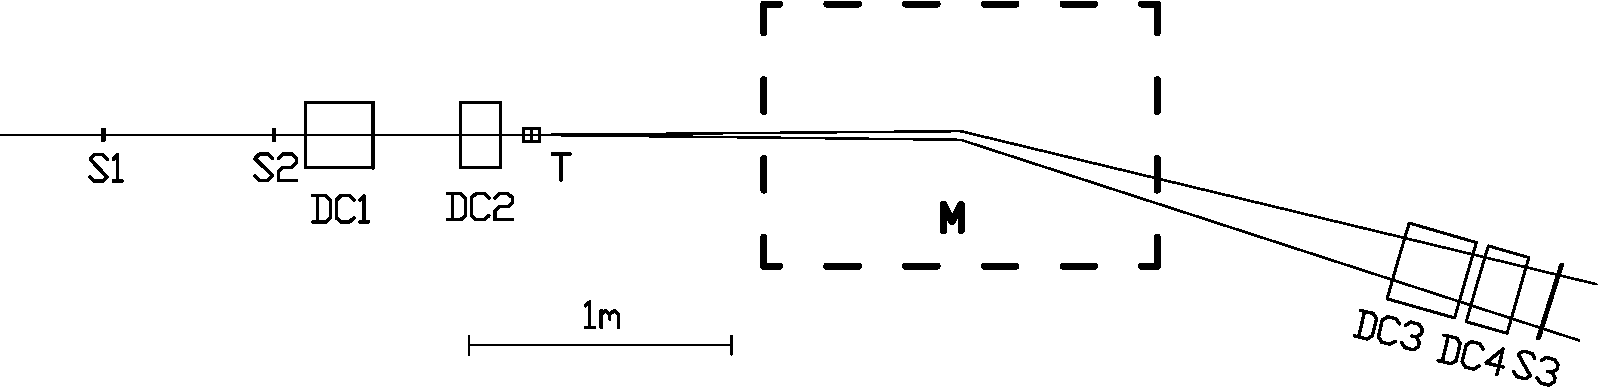
\includegraphics[width=1.00\textwidth]{STRELA_layout.pdf}
  \caption{Schematic layout of the experimental setup to study the \dpchex
    charge exchange channel, consisting of scintillator counters (S1~--~S3),
    drift chambers (DC1 -- DC4), analyzing magnet M and target T.}
  \label{fig:STRELA_layout}
\end{figure*}

Based on the above mentioned ideas and experimental results, obtained using the
1m HBC \cite{gla02,gla08}, the experiment STRELA has been designed and
constructed in the Veksler Baldin Laboratory for High Energy Physics (VBLHEP) of
the Joint Institute for Nuclear Research (JINR) in Dubna with the aim to select
and detect charge exchange events in deuteron proton collisions. The experiment
demands registration of two final state protons with momenta approximately equal
to the half of the primary deuteron beam momenta. STRELA is a typical one arm
magnetic spectrometer, consisting of scintillator detectors (S1 -- S3) used to
trigger the setup, blocks of drift chambers (DC1 -- DC4) used as coordinate
detector, analyzing magnet M and targets (C and CH$_2$), see
Fig.~\ref{fig:STRELA_layout}.

The sensitive areas of the drift chambers are the following: 12.5 $\times$ 12.5
cm$^2$ for DC1, DC2 (small chambers) and 25 $\times$ 25 cm$^2$ for DC3, DC4
(large chambers). The right handed coordinate system has been used, where the
$z$ axis is in the beam direction and $x$ and $y$ axis lie in the plane of the
chambers. Drift chambers contain an (Ar\,+\,CH$_4$) gas mixture and have
alternating, orthogonal $x$ and $y$ coordinate planes. Chambers DC1, DC3, DC4
are equipped with $xy$ wires and DC2 only with $x$ wires. DC1 and DC3 are
composed of 8 sensitive planes ($4y$, $4x$), DC4 is composed of 4 sensitive
planes ($2y$, $2x$) while the DC2 contains 4 sensitive planes ($4x$).

\begin{figure}[t]
  \centering
  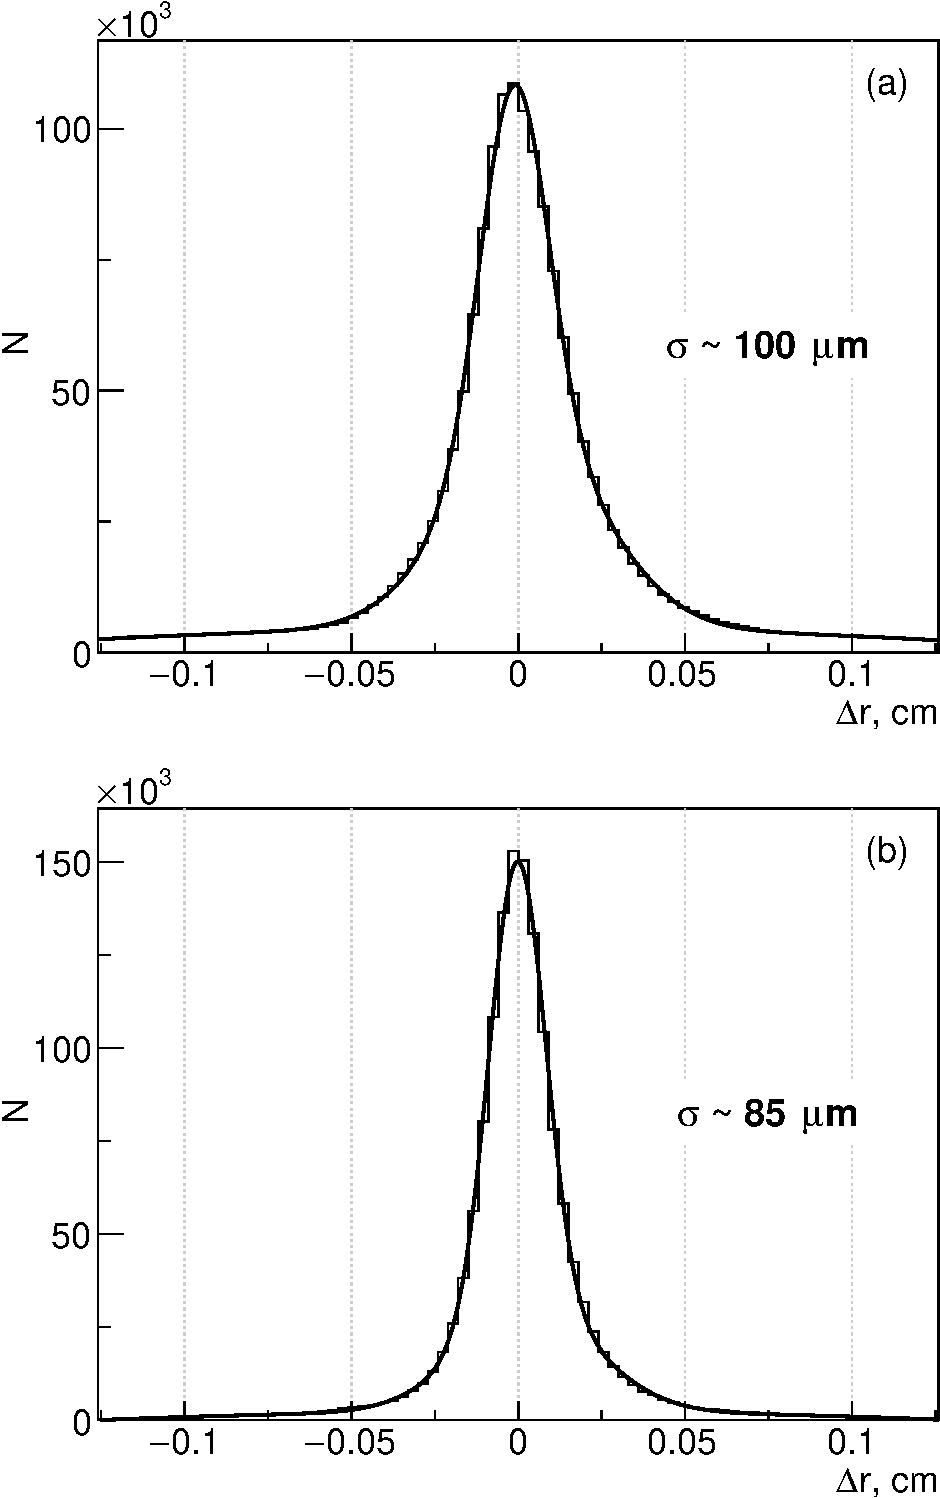
\includegraphics[width=0.47\textwidth]{res_chambers.pdf}
  \caption{Example of distribution of track residuals $\Delta r$ in the $xz$
    plane of drift chambers: (a) small and (b) large. The solid curve is a
    double Gaussian approximation \cite{gla13}.}
  \label{fig:res_chambers}
\end{figure}

The drift length for all chambers is $r_{max} = 21$ mm. The basic
characteristics of the drift chambers have been established from irradiation of
a polyethylene target with a deuteron beam of 3.5 \GeVc momentum. For each wire
the minimal $t_{min}$ and maximal $t_{max}$ drift times have been
determined. The average total drift time was found to be $\sim$~450~ns. In the
track finding procedure the relation between the measured drift time and the
minimal distance from the anode wire to the track plays an important role. To
find the function, transforming the drift time $t$ to radius $r$, also referred
to as $r(t)$ relation, is the central task. This transformation function may
depend on many parameters like: the electric field strength, the gas mixture,
the pressure, the temperature and the drift chamber geometry. For determination
of the transformation function two methods are applied: the linear or quick one,
mainly used for the preliminary results and online monitoring, the second
method, called cumulative or integral one suitable for offline purposes, which
gives the final results. The spatial resolution of the drift chambers used in
the STRELA setup is in the range of $\sim$~80\,--120~$\muup$m
% \muup (or \upmu) not for mathptmx
(Fig.~\ref{fig:res_chambers}). The minimal time between consecutive signals is
$\sim$~50 ns, which corresponds to a minimum distance of $\sim$~2 mm between the
tracks in the drift chamber, which fully satisfies the requirement of the STRELA
experiment. Moreover, the analyzing magnet enhances the space separation of the
recorded protons from the examined reaction. More technical details and the
algorithm of the track reconstruction can be found in \cite{gla13}.

The experimental setup was started by coincidence of two scintillation counters
S1 (dimensions 7.5 $\times$ 7.5 $\times$ 0.5 cm$^3$) and S2 (dimensions diameter
3.0 $\times$ 0.2 cm$^3$). The signals from the XP 2020 photomultipliers are
connected to the shapers with constant fraction timing in order to compensate
the time jitter of the amplitude signal. The time and amplitude information from
the counters is digitized and recorded in each event for the subsequent
monitoring of the counters and the entire trigger system functionality.

The dipole electromagnet 2SP-40, with transverse dimensions 100 $\times$ 30
cm$^2$ and length 150 cm, creates the required magnetic field 0.85 T and serves
as an analyzing magnet. The recorded protons of about the half of the incident
deuteron beam momentum from the examined reaction are bended at 0.289 mrad to
the blocks of large drift chambers (DC3 and DC4) for detection; unscattered
primary deuteron beam does not enter the sensitive areas of these chambers. The
momentum resolution measured with the primary deuteron beam of 3.5 \GeVc is
about 1~\%.

Carbon (C) and polyethylene (CH$_2$) targets are used to extract the $dp$
interaction by subtracting CH$_2$ and C distributions. The volume of the targets
is determined by carbon nuclei equivalent. Their shapes are cylindrical, both
with diameters of 60 mm. The length of targets CH$_2$ and C are 48~mm and 54~mm,
respectively. The density of H nuclei per~cm$^2$ for CH$_2$ target is (4.74
$\pm$ 0.05)$\times$10$^{23}$ cm$^{-2}$.

The measurement was done at the intensities of beam of 2~--~3~$\times$~10$^5$
deuterons per second, duration of the spill was 4~seconds. The deuteron flux
(number of triggers) has been determined by S1 and S2 scintillation counters in
coincidence. This is corrected for the inefficiency of the drift chambers and
admixture of protons in the primary deuteron beam using the empty target
measurements. The value of the correction is different from run to run and is in
the interval 0.85~--~0.89.

The trigger system selects events of the deuteron breakup reaction, where at
least one charged track inclined by magnet reaches the drift chambers DC3 and
DC4. The momenta of the tracks in the event are reconstructed using information
from the magnet and from the drift chambers. Into the analy\-sis only the events
containing two reconstructed tracks are involved.

The detector performance for two-track events was estimated by the use of the
GEANT3 package for transporting the $dp$ interaction products from the 1m HBC
events through the STRELA experimental setup. The plots of momenta
$p_1$~\textit{vs.}~$p_2$ of the two charged particles reaching the DC3 and DC4
chambers are shown in Fig. \ref{fig:p1vsp2_sim}. Simulation including all $dp$
interaction channels (a) and \dpfrag channel only (b). From this comparison and
the fact that 1m HBC is full solid angle detector one can judge that the two
protons of the charge exchange reaction are fully in the detector acceptance.

\begin{figure}[t]
  \centering
  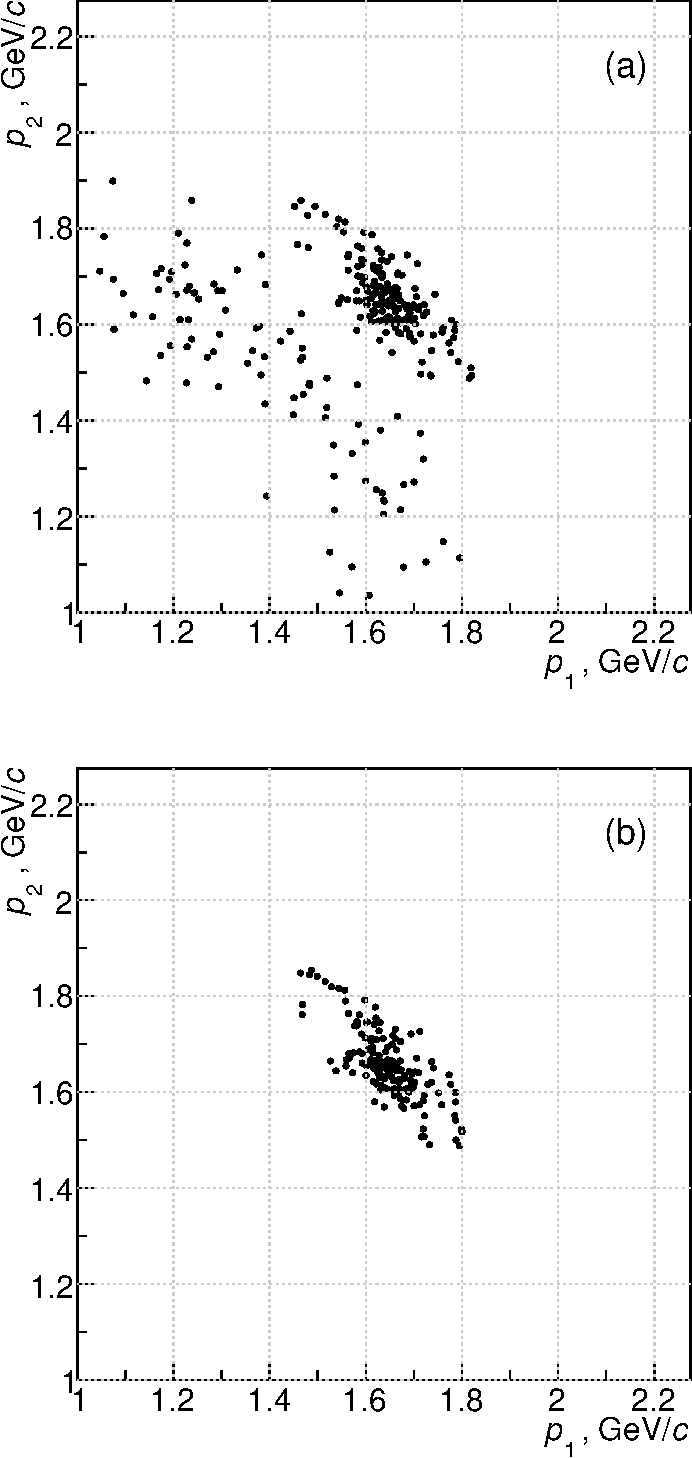
\includegraphics[width=0.43\textwidth]{p1_vs_p2_1.pdf}
  \caption{Plot of the GEANT3 tracked 1m HBC two charged particles momenta $p_1$
    \textit{vs.} $p_2$ from $dp$: all channels (a) and \dpfrag only~(b).}
  \label{fig:p1vsp2_sim}
\end{figure}

\section{Data analysis and experimental results}
The experimental facility has been irradiated in the beam of deuterons with 3.5
\GeVc momenta and approximately milliard triggers were taken. The first step in
the analysis was to decode events. Calibration procedure and the track
reconstruction in the drift chambers transformed the raw data into physical
quantities. For the further processing and physical analysis three track
segments in the $xz$ plane drift chambers were selected: one before the target
and two behind it. The topology of this events is shown in
Fig. \ref{fig:STRELA_layout}. The momentum of the particles (protons) was
determined from the angle of deflection of the charged particle after passing
through the magnet M.

The \dpfrag events reaching the drift chambers DC3 and DC4 are supposed to
contain: two fast protons from the charge exchange reaction \dpchex with momenta
approximately equal to the half of the beam momenta, or a single fast proton
from the charge retention \dpret channel, where the recoil slow proton is
filtered out by the magnet.

In the presented data (Fig. \ref{fig:p1vsp2_exp}) two well-separated areas can
be distinguished as well as in the simulated ones
(Fig.~\ref{fig:p1vsp2_sim}~(a)). The more populated ellipse like area in
Fig. \ref{fig:p1vsp2_sim}~(a) can be ascribed to the charge exchange events if
one compares with the results of simulation in
Fig. \ref{fig:p1vsp2_sim}~(b). This crosschecks the statements made about the
detector acceptance above. The arch like areas in Fig. \ref{fig:p1vsp2_sim}~(a)
and Fig. \ref{fig:p1vsp2_exp} correspond to background two-track events. A
simple cut on the sum of the two reconstructed momenta can remove the events
from the arch like area.

\begin{figure}[h]
  \centering
  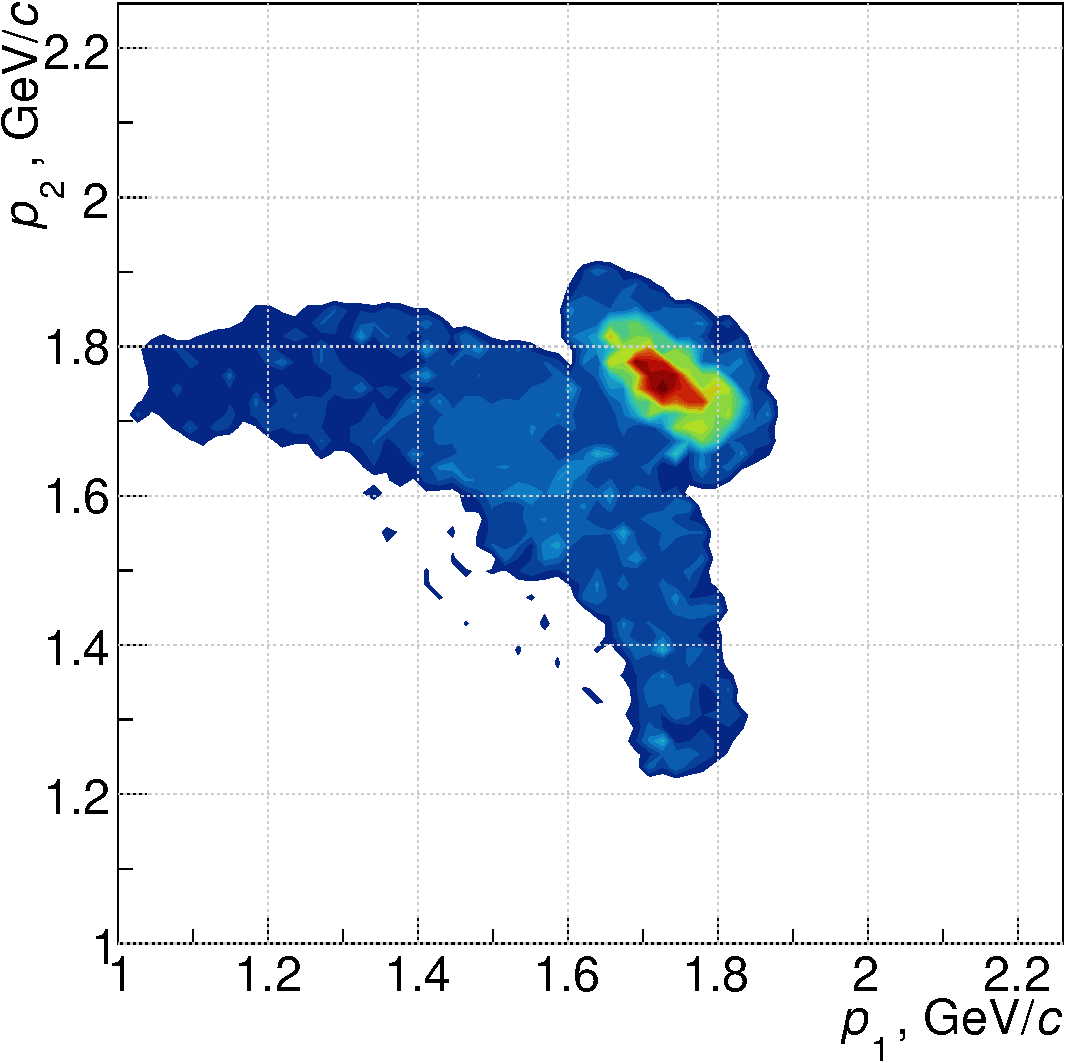
\includegraphics[width=0.43\textwidth]{p1_vs_p2_2.pdf}
  \caption{Plot of the measured momenta $p_1$ \textit{vs.} $p_2$ of the two
    tracks from $d$ + CH$_{2}$ interaction, experimental result.}
  \label{fig:p1vsp2_exp}
\end{figure}

The obtained distribution of the sum of the two charged particles (two protons)
momenta for both CH$_2$ and C targets are displayed in Fig. \ref{fig:p1p2exp},
distinguished by long dashed and dashed lines, respectively. The difference of
the two distributions (full line) shows that the background from C target can be
reduced. The results of simulation shown in Fig.~\ref{fig:p1p2sim} include all
channels of the $dp$ interaction (a) and \dpfrag channel only (b). Note that for
the simulation real events (with relatively small statistics) from the 1m HBC at
the momenta 3.35~\GeVc were used. As one can see, the distribution has a
characteristic peak near the incoming deuteron momentum kinematically associated
with the pair of protons from the \dpfrag reaction (Fig. \ref{fig:p1p2exp}).
Into the further analysis only those events have been included, where the sum of
the two protons momenta is in the interval (3.5 $\pm$ 0.2) \GeVc.

\begin{figure}[t]
  \centering
  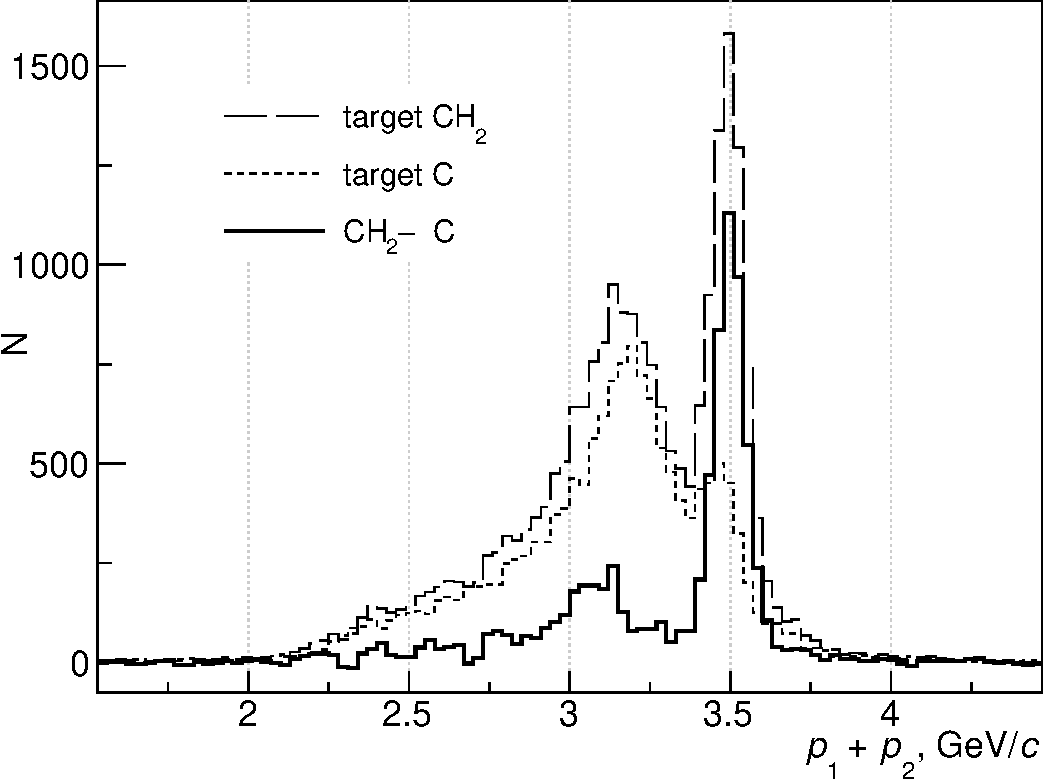
\includegraphics[width=0.43\textwidth]{p1_plus_p2_1.pdf}
  \caption{Distributions of the sum of the two protons momenta from
    $d$~+~CH$_{2}$ and $d$ + C interactions, experimental results: CH$_2$ target
    long dashed line, C target dashed line and their difference full line.}
  \label{fig:p1p2exp}
\end{figure}
\begin{figure}[t]
  \centering
  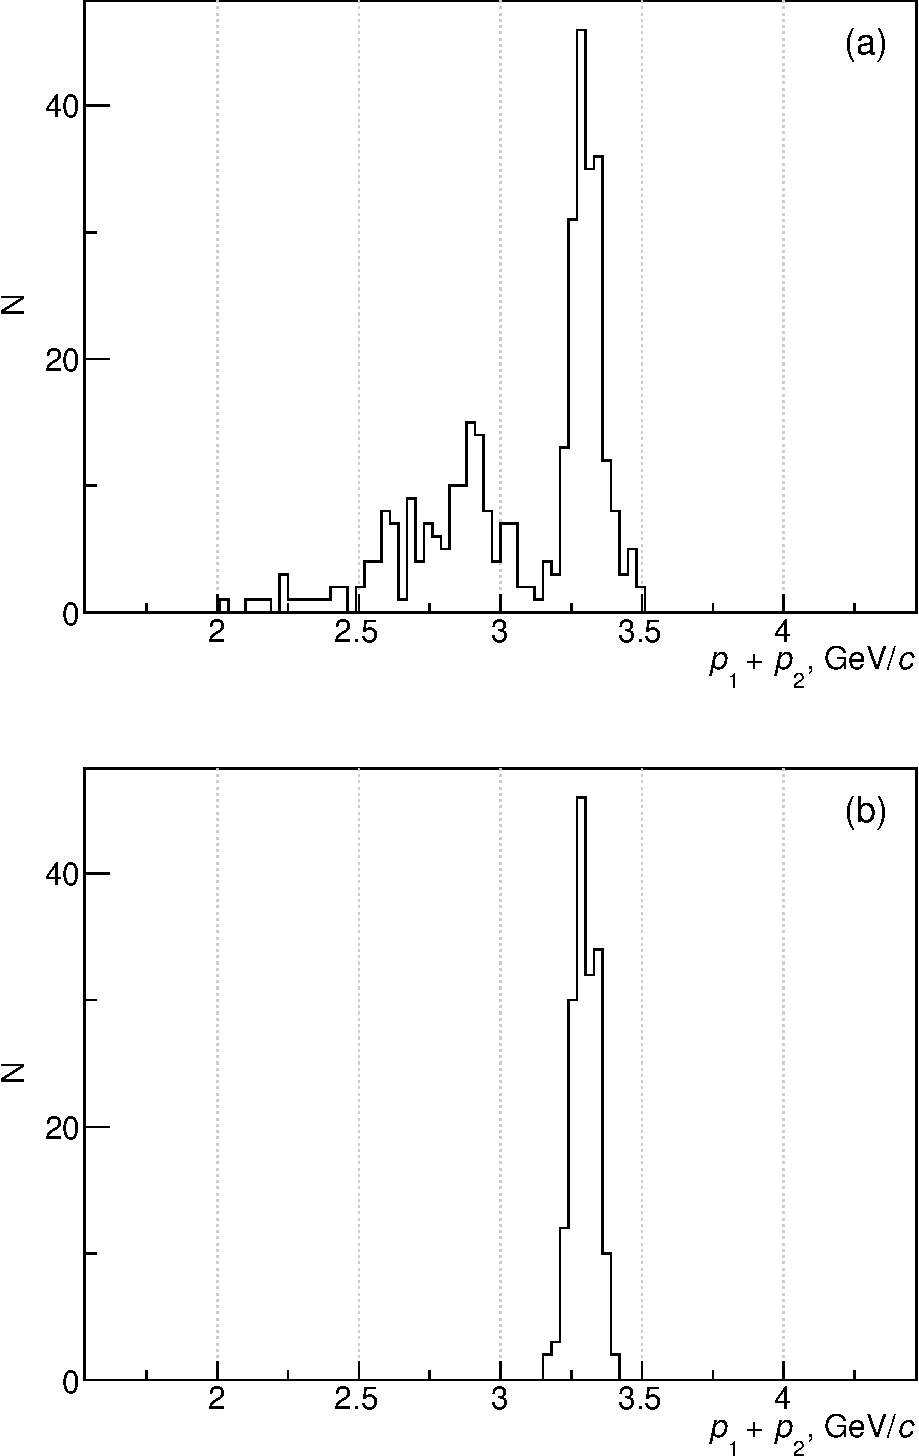
\includegraphics[width=0.43\textwidth]{p1_plus_p2_2.pdf}
  \caption{Distributions of the sum of the two protons momenta from GEANT3
    tracked 1m HBC: $dp$ all channels (a) and \dpfrag channel only (b).}
  \label{fig:p1p2sim}
\end{figure}

The main goal of present experiment is to determine the differential cross
section $(d\sigma/dt)|\,_{t=0}$ of \dpchex, which can only be done as an
extrapolation of the measured data to $|t|\mapsto0$. This can be connected
according to Eq.~\eqref{eq:dp_23np} with the spin-dependent part of the \np
process.

The measured $dN/dt$ distribution of the \dpchex reaction is displayed in
Fig. \ref{fig:dndt} together with the curve corresponding to a fit by
empirically well established expression
\begin{equation}
  dN/dt = a\,\exp(b\,t)\,,
  \label{eq:dndtfit}
\end{equation}
with parameters $a=(435.6 \pm 6.8)$ and $b=(-440.9 \pm 9.1)$. The value
$(dN/dt)|\,_{t=0}$ was transformed to cross section
\begin{equation}
  \frac{d\sigma}{dt}\Big|_{\,t=0} =
  \frac{a}{n\,l\,b_w}\ln\bigg(\frac{N_0}{N_0-N_{rec}}\bigg)\,,
\end{equation}
where $n$ is the number of H nuclei in cm$^{-3}$ in target, $l$ is the target
length in cm, $b_w$ is the histogram bin width. The number of reconstructed two
proton events $N_{rec}$ and the number of incoming deuterons $N_0$ were
corrected for the efficiency of chambers.

\begin{figure}[h]
  \centering
  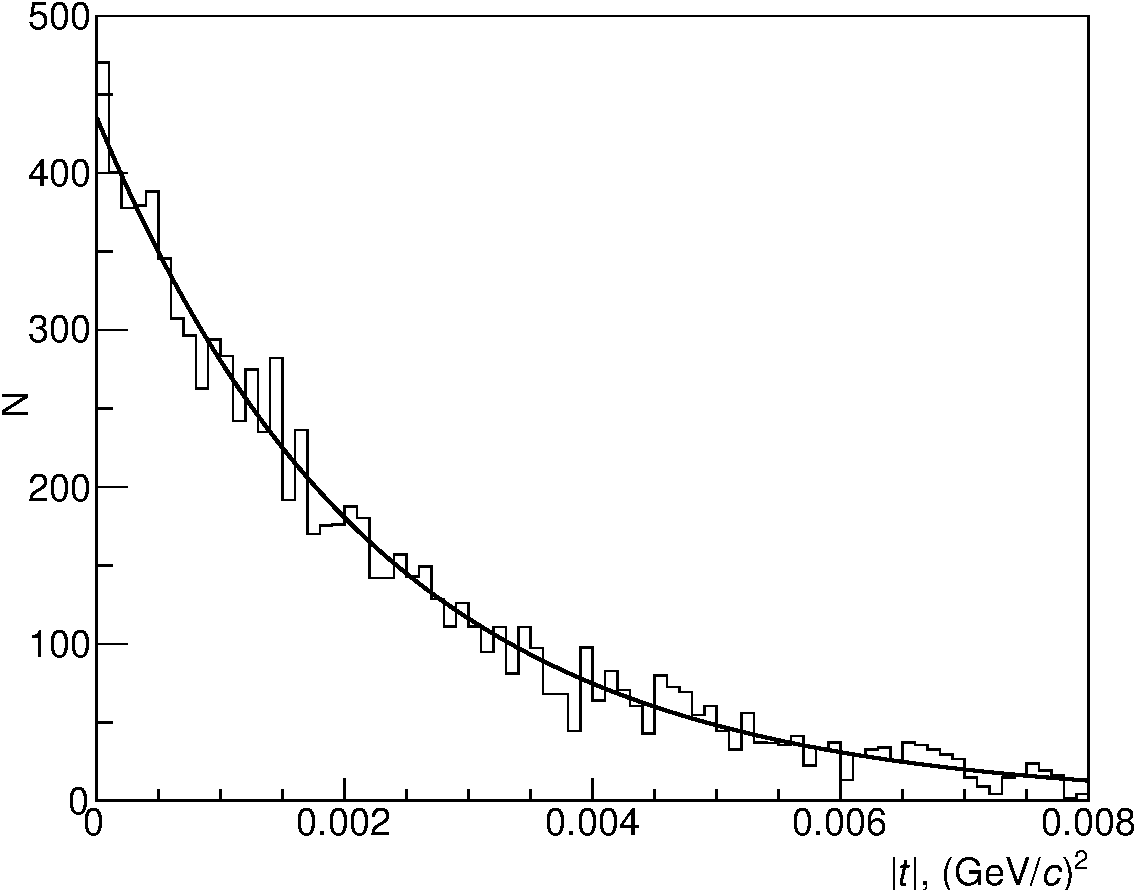
\includegraphics[width=0.48\textwidth]{dp_dN.pdf}
  \caption{Differential distribution $dN/dt$ of the \dpchex reaction. The solid
    line is approximation by Eq. \eqref{eq:dndtfit}.}
  \label{fig:dndt}
\end{figure}

The value $(dN/dt)|\,_{t=0}=(435.6\,\pm\,6.8)$ N$/$(\GeVc)$^{\,2}$ corresponds
to the charge exchange reaction differential cross section
$(d\sigma/dt)|\,_{t=0}=(30.56\,\pm\,0.48$) mb$/$(\GeVc)$^{\,2}$.
% 3x artificial a thin space (Overfull \hbox)
The quoted \,error is statistical \,only. \,Systematic uncertainties which
affect the overall normalization of the cross sections have been estimated to be
about 5~\%. This uncertainty stems mainly from the deuteron flux determination.
The uncertainty from the target thickness and the histogram bin width are
relatively small.

The obtained charge exchange differential cross section on the deuteron at $t=0$
was compared with the available data from \np reaction at the same interpolated
energy from published data. The closest energy data comes from measurements made
at the SATURN accelerator \cite{biz75,bys78}. Unlike to the other similar
experiments, Bizard et al. \cite{biz75} used quasi monochromatic neutrons from
accelerated deuteron stripping with a momentum spread of~5~\%. New data about
\np scattering at the momenta of incident quasi monochromatic neutrons at 1.43,
2.23 and 5.20 \GeVc have been obtained in \cite{tro14}.

The values of $(d\sigma/dt)|\,_{t=0}$ of \np reaction as a function of the
incident momenta is shown in Fig. \ref{fig:npsigma}. Each individual
differential cross sections from Bizard et al. \cite{biz75} are transformed into
$d\sigma/dt$ versus $t$ in the region of momenta 1.4~--~2.0 \GeVc and
extrapolated at each momentum to $t=0$ by fitting the expression
$d\sigma/dt = a\,\exp(b\,t + c\,t^2)$. This reference dependence has already
been used in \cite{gla08}.

\begin{figure}[h]
  \centering
  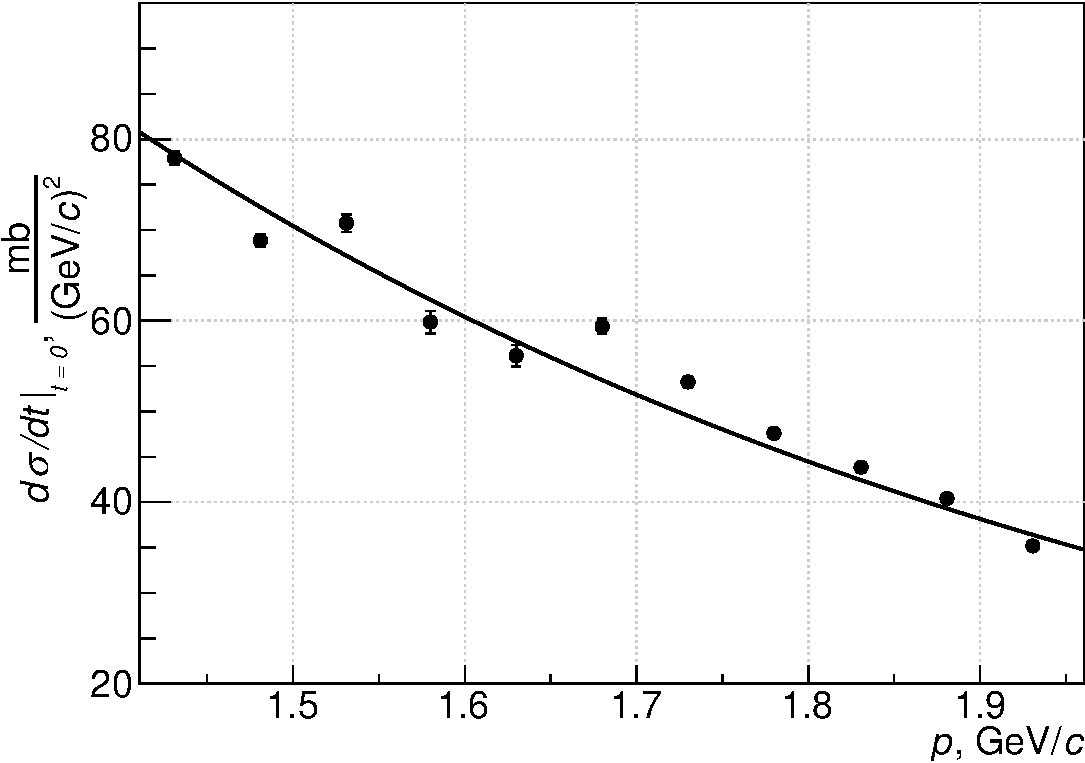
\includegraphics[width=0.48\textwidth]{np_dSigma.pdf}
  \caption{The dependence of the $(d\sigma/dt)|\,_{t=0}$ for the \np reaction on
    the beam momentum. The data points are computed from the experimental
    results \cite{biz75}. The solid curve is a simple exponential fit to the
    data points.}
  \label{fig:npsigma}
\end{figure}

To determine the $(d\sigma/dt)|\,_{t=0}$ of the \np reaction at ``our incident''
proton momentum of 1.75 \GeVc per nucleon, an exponential fit is made to the
results of Fig. \ref{fig:npsigma}, which gives the following value of
$(d\sigma/dt)|\,_{t=0} = (48.0\,\pm\,0.2$) mb$/$(\GeVc)$^{\,2}$. The
systematical error due to fit procedure is approximately 5~\%. The obtained
value will be related to the estimated differential cross section of the quasi
elastic \dpchex charge exchange at $t=0$ from our experiment.

One can introduce the ratio of the differential cross sections for the forward
scattering (charge exchange) on the deuteron and proton
\begin{equation}
  \begin{split}
    R_{\np} &= \frac{(d\sigma/dt)_{\dpchex}}{(d\sigma/dt)_{\np}} \\
    &= 0.64 \pm 0.01\,\mathrm{(stat.)} \pm 0.04\,\mathrm{(syst.)}.
  \end{split}
\end{equation}
Under the assumption Eq. \eqref{eq:dp_23np} and Eq. \eqref{eq:np_sum} stated
above this, $R_{\np}$ can be related to
\begin{equation}
  R_{\np} = \frac{2}{3}\,\frac{(d\sigma/dt)^{SD}_{\np}}{(d\sigma/dt)_{\np}}
\end{equation}
and accordingly the contribution of the spin-independent part, as a ratio of the
two parts of the elastic \np charge exchange cross section, has been obtained as
\begin{equation}
  \begin{split}
    R^{\,ID}_{\np} &= \frac{(d\sigma/dt)^{SI}_{\np}}{(d\sigma/dt)^{SD}_{\np}}
    = \frac{2}{3\,R_{\np}} \ - \ 1 \\
    &= 0.05 \pm 0.02\,\mathrm{(stat.)} \pm 0.07\,\mathrm{(syst.)}.
  \end{split}
\end{equation}
It should be emphasized that the obtained contribution, of course, depends on
the elementary \np charge exchange cross section which is taken from another
experiment and on the systematical errors of approximately 5~\% which is due to
the fit procedure. Preliminary data published in \cite{bas14,bas16} are not
contradicting the presented results.

\section{Conclusion and outlook}
The spectrometric complex STRELA has been proposed and realized to study the
charge exchange reaction in unpola\-rized deuteron beam. The value of the charge
exchange reaction \dpchex differential cross section
$(d\sigma/dt)|\,_{t=0}=(30.56\,\pm\,0.48$) mb$/$(\GeVc)$^{\,2}$ has been
established at 1.75 \GeVc per nucleon. This value agrees with the differential
cross section $(d\sigma/dt)|\,_{t=0}=(30.2\,\pm\,4.1$) mb$/$(\GeVc)$^{\,2}$
determined by means of the one meter hydrogen bubble chamber at 1.675 \GeVc per
nucleon. The obtained ratio of the charge exchange differential cross sections
at $t=0$ for \dpchex and that of \np reaction
$R_{\np} = 0.64 \pm 0.01\,\mathrm{(stat.)} \pm 0.04\,\mathrm{(syst.)}$ testifies
the prevailing contribution of the spin-dependent part to the \np scattering.
This conclusion is in accordance with \cite{gla08}, where the quantities are
published with considerably large errors. For illustration of the improvement in
this experiment one can quote, \textit{e.g.}, the
$R^{\,ID}_{\np} = 0.21 \pm 0.17$ \cite{gla08} and the present ratio
$R^{\,ID}_{\np} = 0.05 \pm 0.02\,\mathrm{(stat.)} \pm 0.07\,\mathrm{(syst.)}$.

In the region above 1 \GeV Delta-Sigma group published the
$R_{dp}(0) = (d\sigma/dt)_{\,nd} / (d\sigma/dt)_{\,np}$ ratios
\cite{sha09,sha09_2,shi11} at seven values of the neutron energies
$T_n = 0.5 - 2.0$ \GeV. Both $nd \rightarrow p(nn)$ and \np reactions were
detected in the same experiment. The reported contributions of the non-flip to
flip ratio in the \np charge exchange are estimated between 0.551 and 0.589
depending on energy. The value of $R_{dp}(0) = 0.553 \pm 0.026$ at 1.0 \GeV
\cite{sha09} is within the experimental uncertainties consistent with our
result. The experiment with monochromatic fast deuterons is more rational in
respect to the analysis of experimental data, \textit{e.g.} STRELA, because the
two secondary protons, products of the \dpchex channel, are fast moving in the
forward direction at small angles, and so they are easily detectable.

In the works \cite{chi09,mch13} the \dpfrag reaction as was used to study
neutron proton charge exchange amplitudes on the ANKE spectrometer at the COSY
storage ring at deuteron energies of 0.6, 0.8, 0.9 and 1.135 \GeV per nucleon.
A rich set of data has been obtained on the differential cross section, vector
and tensor analyzing powers as well as on the spin correlations of the charge
exchange reaction. The whole set of data allowed to draw a conclusion on the
individual amplitudes of the \dpchex scattering. On the other hand, the
spin-independent amplitude $\alpha$, whose magnitude can only be estimated by
comparing the deuteron data with the free \np differential cross section, is
absent.

So, to extend the studies to higher energies on STRELA setup is acceptable and
the preparation is in progress.

\begin{acknowledgements}
  The authors are grateful to the JINR VBLHEP directorate for supporting the
  experiment and the Nuclotron accelerator team for providing the beam. This
  research was supported by the Ministry of Education, Science, Research and
  Sport of the Slovak Republic (VEGA Grant No.~1/0113/18).
\end{acknowledgements}

\begin{thebibliography}{99}
\bibitem{pom51}
  I. Pomeranchuk, Sov. JETF \textbf{21}, 1113 (1951)
\bibitem{chew51}
  G.F. Chew, Phys. Rev. \textbf{84}, 710 (1951)
\bibitem{mig55}
  A.B. Migdal, J. Exp. Theor. Phys. (in Russian) \textbf{28}, 3 (1955)
\bibitem{pom51_2}
  I. Pomeranchuk, Dokl. Akad. Nauk (in Russian) LXXVIII, 249 (1951)
\bibitem{lap57}
  L.I. Lapidus, J. Exp. Theor. Phys. (in Russian) \textbf{32}, 1437 (1957)
\bibitem{dea72}
  N.W. Dean, Phys. Rev. D \textbf{5}, 1661 (1972)
\bibitem{dea72_2}
  N.W. Dean, Phys. Rev. D \textbf{5}, 2832 (1972)
\bibitem{ala75}
  B.S. Aladashvili et al., Nucl. Phys. B \textbf{92}, 189 (1975)
\bibitem{ala75_2}
  B.S. Aladashvili et al., Nucl. Phys. B \textbf{86}, 461 (1975)
\bibitem{bug87}
  D.V. Bugg, C. Wilkin, Nucl. Phys. A \textbf{167}, 575 (1987)
\bibitem{led04}
  R. Lednicky, V.L. Lyuboshitz, V.V. Lyuboshitz, Proc. ISHEPP XVI, 199,
  Dubna (2004)
\bibitem{gla02}
  V.V. Glagolev et al., Eur. Phys. J. A \textbf{15}, 471 (2002)
\bibitem{gol66}
  M. Goldberger, K. Watson, Collision Theory, Wiley, New York (1966)
\bibitem{gla08}
  V.V. Glagolev et al., Cent. Eur. J. Phys. \textbf{6}, 781 (2008)
\bibitem{gla13}
  V.V. Glagolev et al., Instrum. Exp. Tech. \textbf{56}, 387 (2013)
\bibitem{sha09}
  V.I. Sharov et al., Eur. Phys. J. A \textbf{39}, 267 (2009)
\bibitem{sha09_2}
  V.I. Sharov et al., Phys. At. Nucl. \textbf{72}, 1007 (2009)
\bibitem{shi11}
  R.A. Shindin et al., Phys. Part. Nucl. Lett. \textbf{8}, 90 (2011)
\bibitem{chi09}
  D. Chiladze et al., Eur. Phys. J. A \textbf{40}, 23 (2009)
\bibitem{mch13}
  D. Mchedlishvili et al., Eur. Phys. J. A \textbf{49} (2013)
\bibitem{biz75}
  G. Bizard et al., Nucl. Phys B \textbf{85}, 14 (1975)
\bibitem{bys78}
  J. Bystricky, F. Lehar, Nucleon-Nucleon Scattering data, Karlsruhe:
  Fachinformationszentrum, 521, (1978)
\bibitem{tro14}
  Yu.A. Troyan et al., Phys. Part. Nucl. Lett. \textbf{11}, 101 (2014)
\bibitem{bas14}
  S.N. Basilev et al., PoS (Baldin ISHEPP XXII), 137, 2014
\bibitem{bas16}
  S.N. Basilev et al., J. Phys. Conf. Ser. \textbf{678}, 012040, 2016
\end{thebibliography}

\end{document}
